\section{Introduction}

% Basic stuff to talk about in this report
%   - Finding inertia
%       -> Through solidworks
%       -> Experimentally
%   - Control design
%       -> Controller gain values
%       -> Pole-zero plot
%       -> Design for overshoot and settling time
%   - Simulation
%       -> Position control with realistic model
%       -> Real parameters
%   - Amplifier compensation
%

Controller design and simulation is a critical stage in the development of the system as a whole.
% 'the system' - bad
This report details four major steps associated with the design process.
First, determination of accurate model and system parameters; specifically truss inertia.
Second, choice of PID controller gains using the mathematical system model based on specifications for maximum overshoot and settling time.
Third, system simulation to verify and tune controller parameters.
Finally, amplifier control convert the PID output signal to motor voltage accurately.
 
 %\begin{figure}[ht]
 %   \centering
%	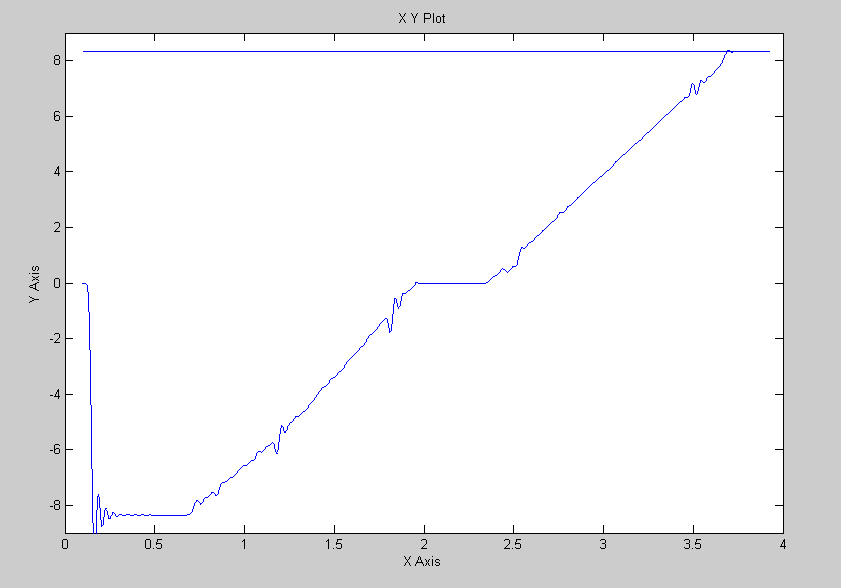
\includegraphics[width=.70\textwidth]{images/InputVsOutputResistive.PNG}
%    \caption{Temp Figure}
%    \label{fig:TEMP}
%\end{figure}


